\begin{figure}
  \centering
  \captionsetup{justification=centering}
  \begin{subfigure}[b]{0.4\linewidth}
    \label{subfig:top_view}
    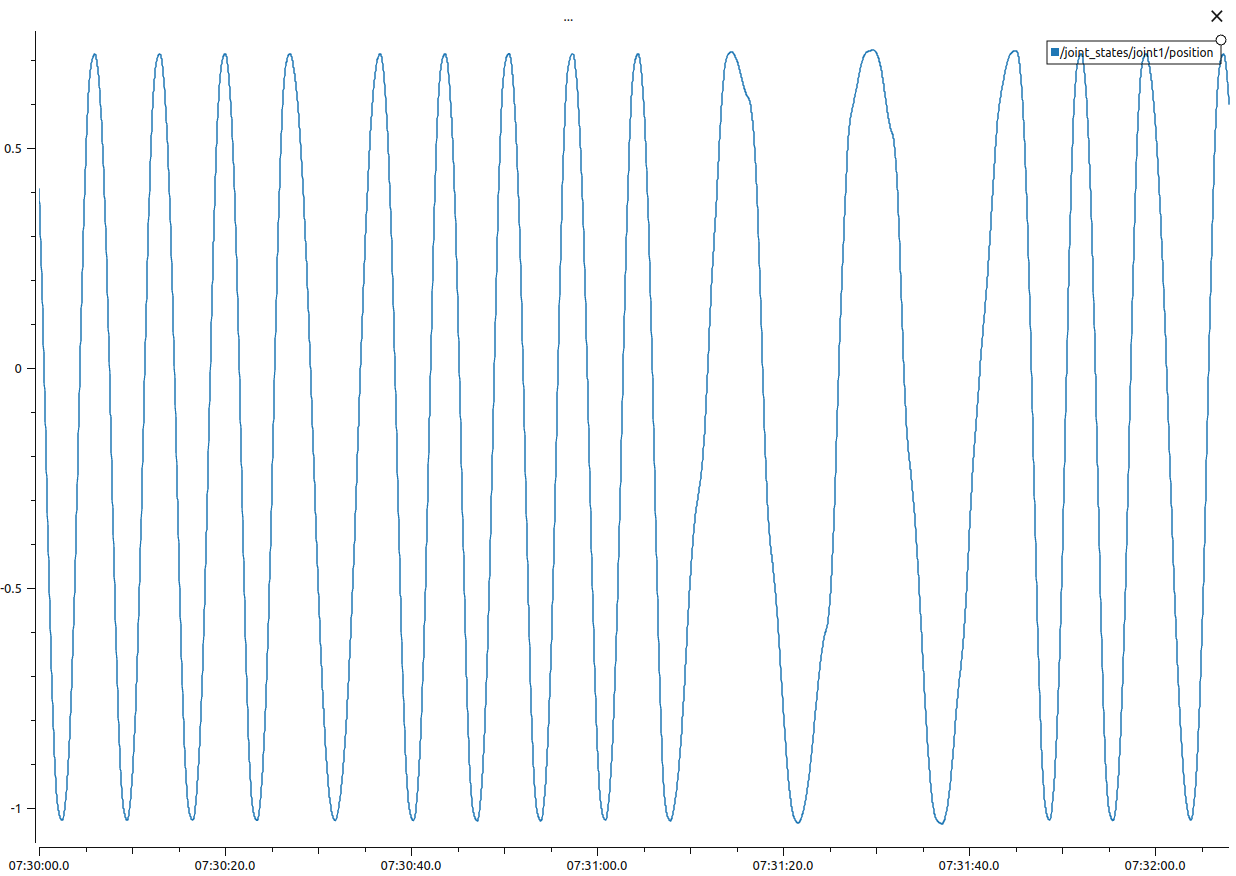
\includegraphics[width=\linewidth]{reaction_joint1.png}
     \caption{}
  \end{subfigure}
  \begin{subfigure}[b]{0.4\linewidth}
    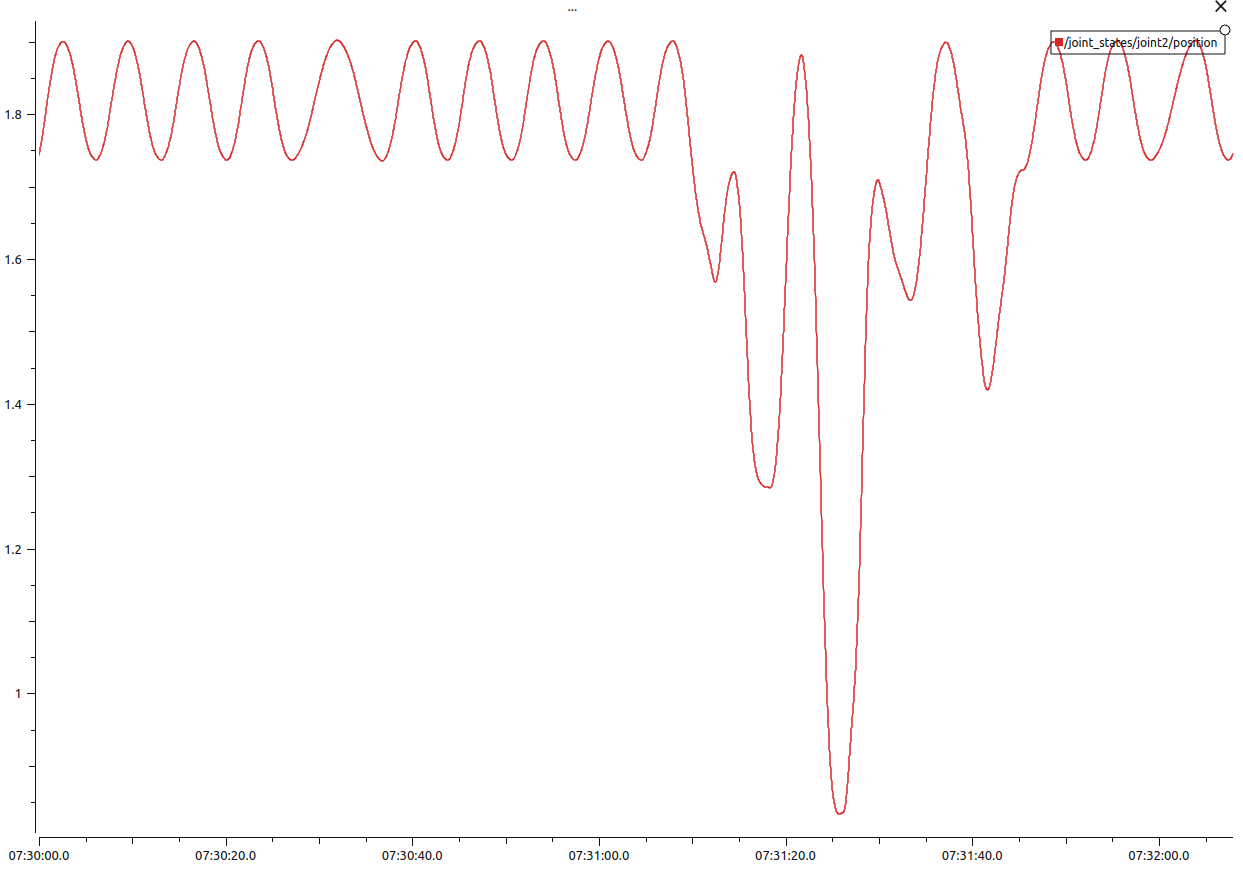
\includegraphics[width=\linewidth]{reaction_joint2.png}
    \caption{}
  \end{subfigure}
  \begin{subfigure}[b]{0.4\linewidth}
    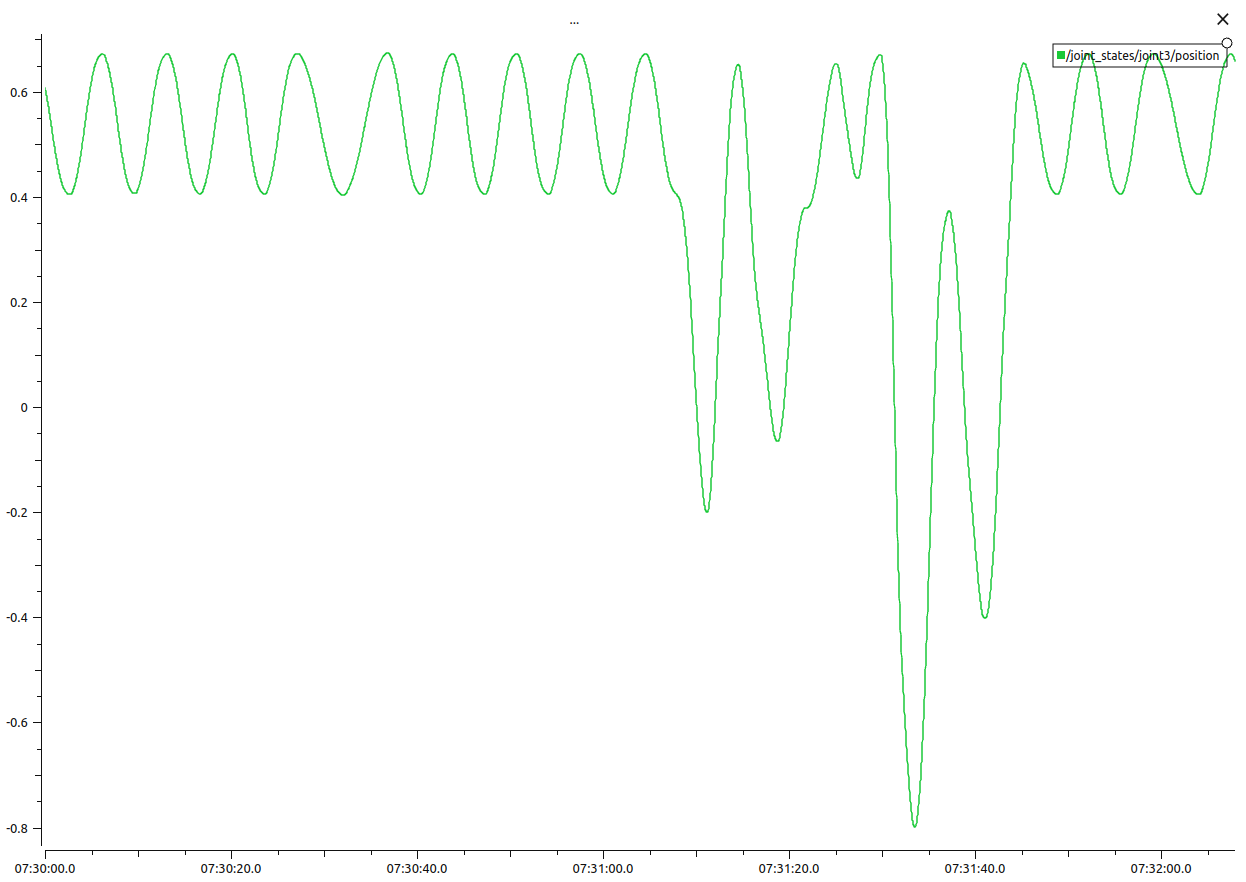
\includegraphics[width=\linewidth]{reaction_joint3.png}
    \caption{}
  \end{subfigure}
  \begin{subfigure}[b]{0.4\linewidth}
    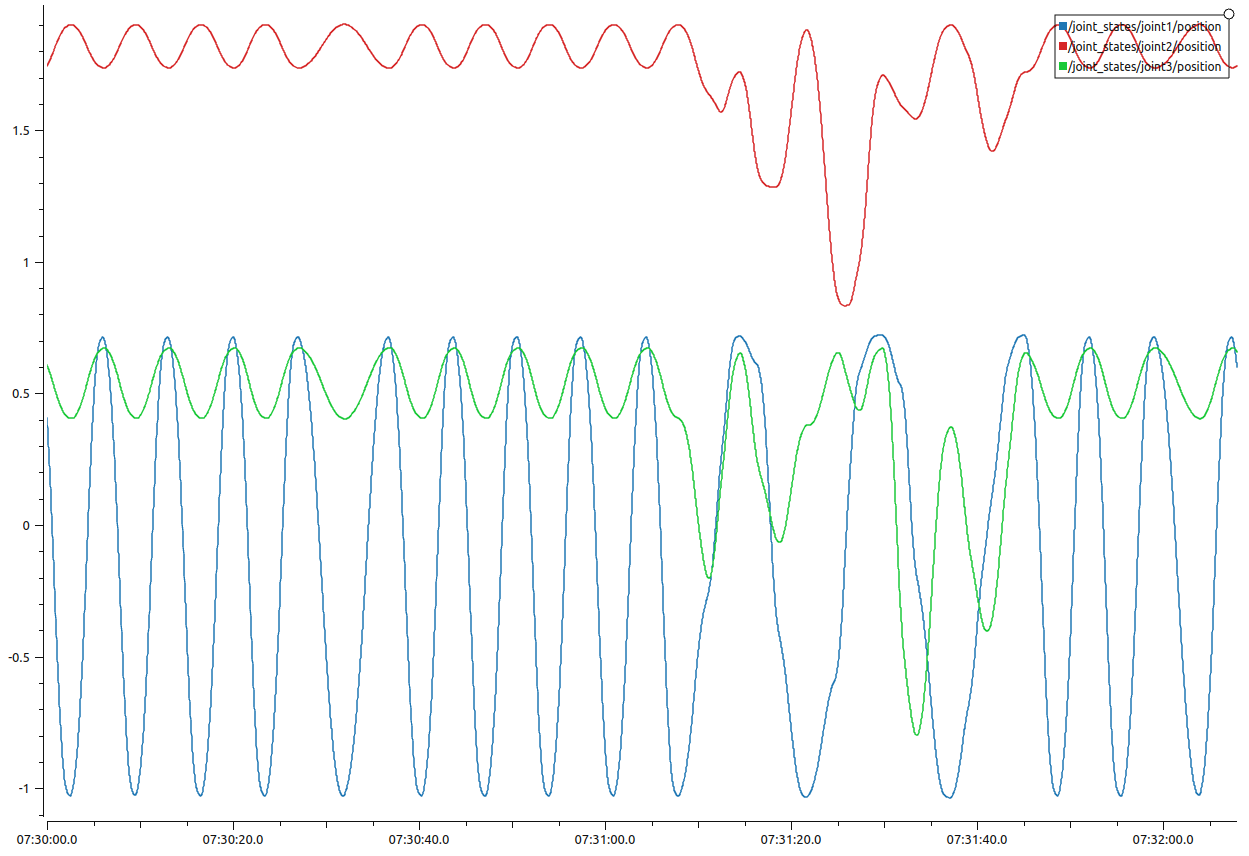
\includegraphics[width=\linewidth]{reaction_joint123.png}
    \caption{}
  \end{subfigure}

  \caption{Reaction from $joint_1, joint_2, joint_3$ shows that the planner
   together with the cycle space behave reactively towards the moving object. No rapid movement or rate on the last three joints on \rimini}
  \label{fig:reaction_joint}
\end{figure}
